\documentclass{beamer}
\usetheme{Madrid}
\colorlet{beamer@blendedblue}{green!40!black}
\setbeamertemplate{caption}[numbered]
\usepackage{amssymb, amsmath, amsthm}
\usepackage{physics, siunitx}
\usepackage{float, subcaption, graphicx}
\usepackage{hyperref}

\title{Chapter 4 - Confinement}
\author{Hunt Feng\inst{1}}
\institute[Usask]
{
	\inst{1}%
	Faculty of Physics And Engineering Physics\\
	University of Saskatchewan
}
\date{\today}

%%%%%%%%%%%%%%%%%%%%
% section page 
%%%%%%%%%%%%%%%%%%%%
\AtBeginSection[]
{
	\begin{frame}{Outline of Presentation}
		\tableofcontents[currentsection]
	\end{frame}
}

\begin{document}
%%%%%%%%%%%%%%%%%%%%
% title and TOC
%%%%%%%%%%%%%%%%%%%%
\maketitle
\begin{frame}{Outline of Presentation}
	\tableofcontents
\end{frame}

%%%%%%%%%%%%%%%%%%%%
% contents 
%%%%%%%%%%%%%%%%%%%%
\section{Transport}
\begin{frame} {Resistive Plasma Diffusion}
  \begin{itemize}
    \item Resistive diffusion coefficient
          \[ D = \frac{\eta_\perp\beta}{2\mu_0} \sim \frac{\rho}{\tau} = D_c \]
          where $\rho$ and $\tau$ are step length and step time from classical random walk model.
    \item Resistive diffusion gives diffusion coefficient similar to classical result $D_c$.
  \end{itemize}
\end{frame}

\begin{frame} {Banana/Plateau/Pfirsch-Schl\"{u}ter Transport}
  \begin{itemize}
    \item Classical diffusion coefficient is $ D_{c} = \rho^{2}\nu $, where $\rho$ is the random walk length, and $\nu$ is the collision frequency.
    \item Plateau diffusion coefficient
          \[ D \sim \frac{v_{\parallel}}{v_{T}}v_{d}^{2} \frac{Rq}{v_{\parallel}} \sim \frac{v_{T}q}{R}\rho^{2} \]
  \end{itemize}

  \begin{figure}
    \centering
    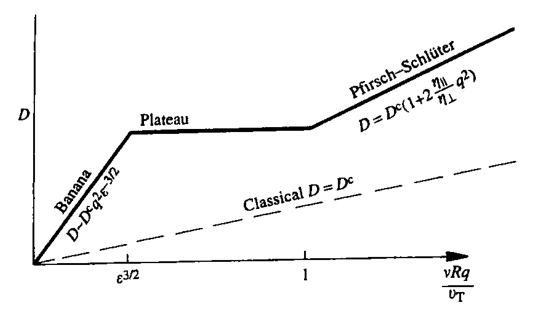
\includegraphics[width=0.6\textwidth]{figures/plateau-transport.png}
    \caption{Variation of diffusion coefficient with collision frequency.}
    \label{fig:plateau-transport}
  \end{figure}
\end{frame}

\begin{frame} {Ripple Transport}
  \begin{itemize}
    \item The finite number of toroidal field coils destroys the perfect axisymmetry of the device.
    \item Particles are trapped / lose energies to the "ripple well".
  \end{itemize}
  \begin{figure}
    \centering
    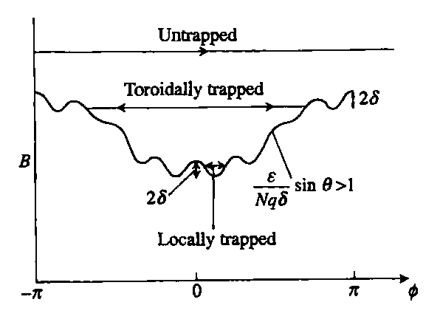
\includegraphics[width=0.5\textwidth]{figures/ripple-transport.png}
    \caption{Variation of magnetic field strength along a field line in a tokamak with a rippled field, and the resulting types of particle trapping.}
    \label{fig:ripple-transport}
  \end{figure}
\end{frame}

\section{Confinement Modes}
\begin{frame} {Confinement Modes}
    \begin{itemize}
        \item \textbf{Ohmically heated plasmas}:
              \[ \tau_E = 0.07(n/10^{20})aR^2q\]
              Confinement increases as density increases.
        \item \textbf{L-mode}:
              \[ \tau_E^{ITER89-P} = 0.048\frac{I^{0.85}R^{1.2}a^{0.3}\kappa^{0.5}(n/10^{20})^{0.1}B^{0.2}A^{0.5}}{P^{0.5}} \]
              Confinement drops and heating power $P$ increases.
        \item \textbf{H-mode}:
              \[ \tau_{Th}^{ITER H93-P} = 0.053\frac{I^{1.06}R^{1.9}a^{-0.11}\kappa^{0.66}(n/10^{20})^{0.17}B^{0.32}A^{0.41}}{P^{0.67}} \]
              $\tau_{Th}$ refers to confinement time for the thermal part of the plasma energy. It is valid without edge localized modes (ELMs).
    \end{itemize}
\end{frame}

\begin{frame} {H-modes}
    \begin{itemize}
        \item H-mode has good confinement.
        \item At the edge, shape density gradient is steep.
        \item Transport barrier at the edge is developed.
    \end{itemize}
    \begin{figure}
        \centering
        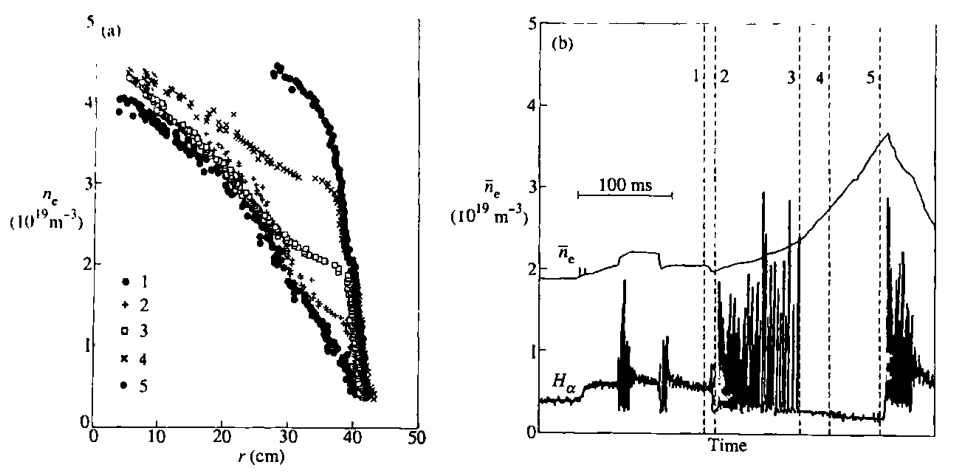
\includegraphics[width=0.7\textwidth]{figures/h-mode.png}
        \caption{Sequence of density profiles measured on ASDEX through and following an L-H transition. The profiles in (a) are at the times shown in (b), which gives the time dependence of $\bar{n}_e$ and the $H_\alpha$ signal.}
        \label{fig:h-mode}
    \end{figure}
\end{frame}

\begin{frame} {Internal Transport Barriers}
    \begin{figure}
        \centering
        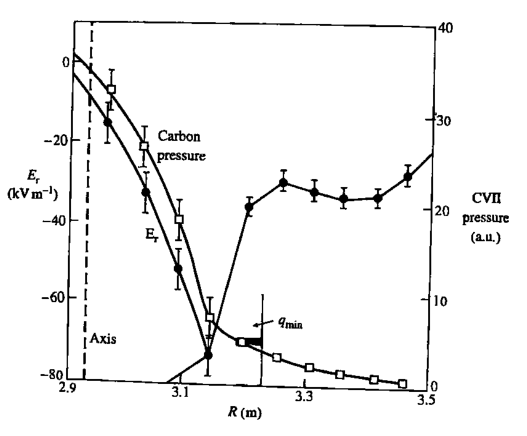
\includegraphics[width=0.5\textwidth]{figures/internal-transport-barrier.png}
        \caption{Radial electric field and carbon pressure profiles in an ERS discharge in TFTR. Fluctuations and turbulent fluxes are reduced inside the transport barrier near the minimum in $q$. Correspondingly, the carbon pressure profile has a stepper gradient in this region. The transport barrier is associated with a rapidly varying profile of $E_r$.}
        \label{fig:internal-transport-barrier}
    \end{figure}
\end{frame}

\section{Fluctuations}
\begin{frame} {Fluctuations}
    \begin{itemize}
        \item Turbulent fluctuations produce an $\mathbf{E\times B}$ drift velocity $\delta v_\perp = \delta E_\perp/B$.
        \item With density fluctuation $\delta n$, the convective particle flux is
              \[ \Gamma = \expval{\delta v_\perp\delta n} \]
              Average is taken over the flux surface.
        \item With magnetic fluctuations $\delta \mathbf{B}$, the flux is
              \[ \Gamma_j = \frac{n}{B}\expval{\delta v_{\parallel j}\delta B_r} \]
    \end{itemize}
\end{frame}

\begin{frame} {Fluctuations and $\tau_E$}
    \begin{figure}
        \centering
        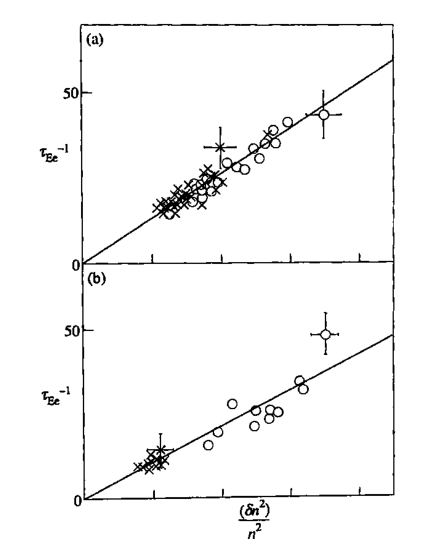
\includegraphics[width=0.35\textwidth]{figures/fluctuations-and-tau-e.png}
        \caption{Measurements from TFR showing a correlation between the level of density fluctuations and the electron energy confinement time (with allowance for the effect of sawtooth oscillations). Figure (a) is for ion cyclotron heating and Fig.(b) is for neutral beam beating. Both figures also give results for ohmic heating.}
        \label{fig:}
    \end{figure}
\end{frame}

\begin{frame} {Fluctuations and L-H Transition}
    \begin{figure}
        \centering
        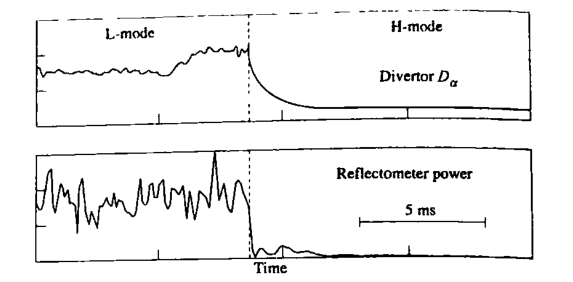
\includegraphics[width=0.7\textwidth]{figures/fluctuations-and-modes.png}
        \caption{Showing the fall of density fluctuations as measured by reflectometry during an L-H transition in DIII-D.}
        \label{fig:fluctuation-and-modes}
    \end{figure}
\end{frame}

\begin{frame} {Turbulence-Induced Transport}
    \begin{itemize}
        \item \textbf{Transport due to electrostatic fluctuations}:
              \[ D = \sum_k \left( \frac{k_\perp\delta\phi_k}{B} \right)^2 \tau_k \]
              We have assumed the fluctuations of electric potential $\delta\phi = \sum_k\delta\phi_ke^{i\mathbf{k\cdot x}}$. The time variation of the fluctuation is characterized by $\tau_k \sim 1/\omega_k$.
        \item \textbf{Transport due to magnetic fluctuations}:
              \[ D_M = \sum_k \frac{k_\perp\omega_k^3}{L_s} \]
    \end{itemize}
\end{frame}

%%%%%%%%%%%%%%%%%%%%
% references
%%%%%%%%%%%%%%%%%%%%
\newpage
\begin{frame}[allowframebreaks]
	All figures are adopted from \cite{wesson_campbell_tokamaks_2011}.
	\bibliographystyle{abbrv}
	\bibliography{../references}
	\nocite{*}
\end{frame}

\end{document}
